\documentclass[12pt,a4paper,openright,twoside]{book}
\usepackage[utf8]{inputenc}
\usepackage{disi-thesis}
\usepackage{code-lstlistings}
\usepackage{notes}
\usepackage{shortcuts}
\usepackage{acronym}

\school{\unibo}
\programme{Corso di Laurea in Ingegneria e Scienze Informatiche}
\title{OpenGL e Vulkan: un caso di studio}
\author{Palazzini Luca}
\date{\today}
\subject{Computer Graphics}
\supervisor{Prof.ssa Damiana Lazzaro}
\session{I}
\academicyear{2024-2025}

\mainlinespacing{1.241}

\begin{document}

% Definition of acronyms
\begin{acronym}[API]
  \acro{API}{Application Programming Interface}
  \acro{PBR}{Physically Based Rendering}
  \acro{CPU}{Central Processing Unit}
  \acro{GPU}{Graphical Processing Unit}
\end{acronym}

\frontmatter\frontispiece

% TODO: Write abstract
\begin{abstract}	
Max 2000 characters, strict.
\end{abstract}

% TODO: Write dedication (optional)
\begin{dedication}
Optional. Max a few lines.
\end{dedication}

% Table of contents
\tableofcontents   
\listoffigures
% TODO: Uncomment when listing added \lstlistoflistings

% Main content
\mainmatter

%----------------------------------------------------------------------------------------
\chapterWithoutNumber{Introduzione}
\label{chap:introduction}
%----------------------------------------------------------------------------------------

\paragraph{Contesto e Motivazioni}
Negli ultimi anni, il campo della grafica computazionale ha visto un'evoluzione significativa delle \emph{Graphics \acs{API}}
verso modelli di programmazione più vicini all'hardware e orientati alle alte prestazioni.  
OpenGL, storicamente una delle \ac{API} più diffuse, offre un modello di programmazione di tipo \emph{high-level}, che
semplifica lo sviluppo ma lascia al driver una gestione implicita di numerosi aspetti, come la sincronizzazione e la
gestione della memoria.  
Vulkan, introdotta dal \emph{Khronos Group} nel 2016, adotta invece un approccio \emph{low-level}, demandand
programmatore un controllo esplicito sulle risorse e sull’esecuzione dei comandi, con l’obiettivo di ridurre l’overhead
del driver e di consentire una migliore parallelizzazione del carico di lavoro.
Lo scopo di questo elaborato è indagare le differenze prestazionali e architetturali tra le due \ac{API}, attraverso
la realizzazione di un motore di rendering capace di utilizzare entrambe le tecnologie.  
Il confronto si concentra in particolare sull’impatto del multithreading in Vulkan rispetto al modello single-thread
tipico di OpenGL, analizzando come la differente gestione della pipeline grafica influisca sulle prestazioni complessive.

\paragraph{Obiettivi}
L’obiettivo principale del lavoro è progettare e sviluppare un motore di rendering scritto in \emph{C++23},
in grado di operare sia con OpenGL 4.6 sia con Vulkan 1.4.
Il motore implementa un approccio di tipo \emph{deferred rendering}, supporta materiali \ac{PBR}, luci direzionali,
puntuali e spot, e include ulteriori passaggi di rendering per particelle e oggetti di debug.
L’architettura segue un paradigma orientato agli oggetti, integrando librerie e framework comuni.
L’obiettivo sperimentale è valutare, a parità di contenuto e condizioni di rendering, l’efficienza delle due API 
in termini di:
\begin{itemize}
    \item tempo medio per frame e frame rate;
    \item utilizzo della \acs{CPU} e della \acs{GPU};
\end{itemize}

\paragraph{Metodo di lavoro}
Il progetto è stato sviluppato con un approccio incrementale, secondo cicli iterativi di implementazione e validazione.  
Dopo la fase di progettazione architetturale, il motore è stato realizzato con un sistema modulare che separa la logica
di rendering dal resto della gestione della scena, consentendo di confrontare in modo diretto i due backend grafici.  
% TODO: mention Sponza scene %
I test prestazionali sono stati condotti su una scena principale, utilizzando diversi hardware, variando numero di luci
e \emph{particle systems}, per misurare in modo oggettivo i benefici derivati dal parallelismo offerto da Vulkan.

\paragraph{Struttura del documento}
Il documento è organizzato come segue:
\begin{itemize}
   \item Il \textbf{Capitolo 1} introduce i concetti fondamentali relativi al rendering, alle \ac{API} grafiche moderne e alle tecniche \ac{PBR} e deferred rendering;
   \item Il \textbf{Capitolo 2} analizza i requisiti del progetto e le scelte progettuali alla base del motore sviluppato;
   \item Il \textbf{Capitolo 3} descrive l’architettura del sistema e i principali componenti software;
   \item Il \textbf{Capitolo 4} illustra l’implementazione e mostra esempi di codice e schermate del motore in funzione;
   \item Il \textbf{Capitolo 5} presenta la valutazione sperimentale, i risultati delle misure e la loro analisi critica.
\end{itemize}

%----------------------------------------------------------------------------------------
\chapter{Background}
\label{chap:background}
%----------------------------------------------------------------------------------------

\section{Pipeline di Rendering}
Il rendering grafico può essere realizzato seguendo approcci diversi. I principali sono il \emph{forward rendering}
e il \emph{deferred rendering}.  
Nel forward rendering, le luci vengono calcolate direttamente durante il rendering di ciascun oggetto, con conseguente
aumento dei costi per scene complesse con molte luci.  
Il deferred rendering separa la fase di geometria da quella di illuminazione, memorizzando informazioni come posizione,
normale e materiali in buffer intermedi (\emph{G-buffer}) per poi eseguire il calcolo della luce in un passaggio successivo.  
\begin{figure}[h!]
    \centering
    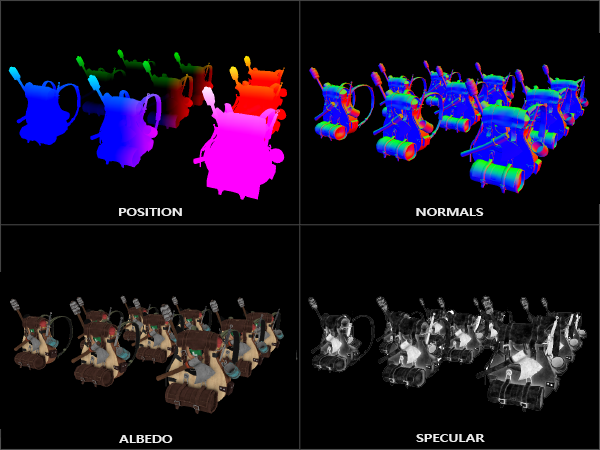
\includegraphics[width=.8\linewidth]{figures/g_buffer_example.png}
    \caption{Esempio di pipeline di deferred rendering from \cite{learnopengl}.}
    \label{fig:deferred-pipeline}
\end{figure}

\section{Physically Based Rendering (\ac{PBR})}
Il \emph{\acl{PBR}} permette una resa più realistica dei materiali basandosi su modelli fisici di illuminazione.  
I materiali sono descritti da parametri quali:
\begin{itemize}
    \item \textbf{Albedo}: colore base del materiale;
    \item \textbf{Roughness}: misura della microfacettatura superficiale;
    \item \textbf{Metallic}: indica la natura metallica del materiale;
    \item \textbf{Normal map}: dettaglio delle normali della superficie.
\end{itemize}

\section{Graphics APIs: OpenGL and Vulkan}

\section{Libraries and Tools}

\section{Related Work}

%----------------------------------------------------------------------------------------
\chapter{Requirements and Analysis}
\label{chap:analysis}
%----------------------------------------------------------------------------------------

\section{Functional Requirements}

\section{Non-functional Requirements}

\section{Constraints}

\section{Evaluation Strategy}

%----------------------------------------------------------------------------------------
\chapter{Design and Architecture}
\label{chap:design}
%----------------------------------------------------------------------------------------

\section{System Overview}

\section{Object-Oriented Design}

\section{Renderer Architecture}

\section{Deferred Rendering Pipeline}

\section{Resource Management}

%----------------------------------------------------------------------------------------
\chapter{Implementation}
\label{chap:implementation}
%----------------------------------------------------------------------------------------

\section{Codebase Structure}

\section{Key Components}

\section{PBR Material System}

\section{Particle Simulation}

\section{Performance GUI}

%----------------------------------------------------------------------------------------
\chapter{Performance Evaluation}
\label{chap:evaluation}
%----------------------------------------------------------------------------------------

\section{Experimental Setup}

\section{Results}

\section{Discussion}

%----------------------------------------------------------------------------------------
\chapterWithoutNumber{Conclusions and Future Work}
\label{chap:conclusions}
%----------------------------------------------------------------------------------------

\paragraph{Summary}

\paragraph{Findings}

\paragraph{Limitations}

\paragraph{Future Work}

% End of thesis
\backmatter

\nocite{*}

\bibliographystyle{alpha}
\bibliography{bibliography}

% TODO: Write acknowledgements (optional)
\begin{acknowledgements}
Optional. Max 1 page.
\end{acknowledgements}

\end{document}
